
%% bare_jrnl.tex
%% V1.3
%% 2007/01/11
%% by Michael Shell
%% see http://www.michaelshell.org/
%% for current contact information.
%%
%% This is a skeleton file demonstrating the use of IEEEtran.cls
%% (requires IEEEtran.cls version 1.7 or later) with an IEEE journal paper.
%%
%% Support sites:
%% http://www.michaelshell.org/tex/ieeetran/
%% http://www.ctan.org/tex-archive/macros/latex/contrib/IEEEtran/
%% and
%% http://www.ieee.org/

% *** Authors should verify (and, if needed, correct) their LaTeX system  ***
% *** with the testflow diagnostic prior to trusting their LaTeX platform ***
% *** with production work. IEEE's font choices can trigger bugs that do  ***
% *** not appear when using other class files.                            ***
% The testflow support page is at:
% http://www.michaelshell.org/te x/testflow/


%%*************************************************************************
%% Legal Notice:
%% This code is offered as-is without any warranty either expressed or
%% implied; without even the implied warranty of MERCHANTABILITY or
%% FITNESS FOR A PARTICULAR PURPOSE! 
%% User assumes all risk.
%% In no event shall IEEE or any contributor to this code be liable for
%% any damages or losses, including, but not limited to, incidental,
%% consequential, or any other damages, resulting from the use or misuse
%% of any information contained here.
%%
%% All comments are the opinions of their respective authors and are not
%% necessarily endorsed by the IEEE.
%%
%% This work is distributed under the LaTeX Project Public License (LPPL)
%% ( http://www.latex-project.org/ ) version 1.3, and may be freely used,
%% distributed and modified. A copy of the LPPL, version 1.3, is included
%% in the base LaTeX documentation of all distributions of LaTeX released
%% 2003/12/01 or later.
%% Retain all contribution notices and credits.
%% ** Modified files should be clearly indicated as such, including  **
%% ** renaming them and changing author support contact information. **
%%
%% File list of work: IEEEtran.cls, IEEEtran_HOWTO.pdf, bare_adv.tex,
%%                    bare_conf.tex, bare_jrnl.tex, bare_jrnl_compsoc.tex
%%*************************************************************************

% Note that the a4paper option is mainly intended so that authors in
% countries using A4 can easily print to A4 and see how their papers will
% look in print - the typesetting of the document will not typically be
% affected with changes in paper size (but the bottom and side margins will).
% Use the testflow package mentioned above to verify correct handling of
% both paper sizes by the user's LaTeX system.
%
% Also note that the "draftcls" or "draftclsnofoot", not "draft", option
% should be used if it is desired that the figures are to be displayed in
% draft mode.
%
\documentclass[journal]{IEEEtran}
%
% If IEEEtran.cls has not been installed into the LaTeX system files,
% manually specify the path to it like:
% \documentclass[journal]{../sty/IEEEtran}





% Some very useful LaTeX packages include:
% (uncomment the ones you want to load)


% *** MISC UTILITY PACKAGES ***
%
%\usepackage{ifpdf}
% Heiko Oberdiek's ifpdf.sty is very useful if you need conditional
% compilation based on whether the output is pdf or dvi.
% usage:
% \ifpdf
%   % pdf code
% \else
%   % dvi code
% \fi
% The latest version of ifpdf.sty can be obtained from:
% http://www.ctan.org/tex-archive/macros/latex/contrib/oberdiek/
% Also, note that IEEEtran.cls V1.7 and later provides a builtin
% \ifCLASSINFOpdf conditional that works the same way.
% When switching from latex to pdflatex and vice-versa, the compiler may
% have to be run twice to clear warning/error messages.






% *** CITATION PACKAGES ***
%
%\usepackage{cite}
% cite.sty was written by Donald Arseneau
% V1.6 and later of IEEEtran pre-defines the format of the cite.sty package
% \cite{} output to follow that of IEEE. Loading the cite package will
% result in citation numbers being automatically sorted and properly
% "compressed/ranged". e.g., [1], [9], [2], [7], [5], [6] without using
% cite.sty will become [1], [2], [5]--[7], [9] using cite.sty. cite.sty's
% \cite will automatically add leading space, if needed. Use cite.sty's
% noadjust option (cite.sty V3.8 and later) if you want to turn this off.
% cite.sty is already installed on most LaTeX systems. Be sure and use
% version 4.0 (2003-05-27) and later if using hyperref.sty. cite.sty does
% not currently provide for hyperlinked citations.
% The latest version can be obtained at:
% http://www.ctan.org/tex-archive/macros/latex/contrib/cite/
% The documentation is contained in the cite.sty file itself.



% *** GRAPHICS RELATED PACKAGES ***
%
\ifCLASSINFOpdf
  \usepackage[pdftex]{graphicx}
  \usepackage{epstopdf}
 \usepackage{amsmath,amssymb,exscale}

  % declare the path(s) where your graphic files are
  % \graphicspath{{../pdf/}{../jpeg/}}
  % and their extensions so you won't have to specify these with
  % every instance of \includegraphics
  % \DeclareGraphicsExtensions{.pdf,.jpeg,.png}
\else
  % or other class option (dvipsone, dvipdf, if not using dvips). graphicx
  % will default to the driver specified in the system graphics.cfg if no
  % driver is specified.
  % \usepackage[dvips]{graphicx}
  % declare the path(s) where your graphic files are
  % \graphicspath{{../eps/}}
  % and their extensions so you won't have to specify these with
  % every instance of \includegraphics
  % \DeclareGraphicsExtensions{.eps}
\fi
% graphicx was written by David Carlisle and Sebastian Rahtz. It is
% required if you want graphics, photos, etc. graphicx.sty is already
% installed on most LaTeX systems. The latest version and documentation can
% be obtained at: 
% http://www.ctan.org/tex-archive/macros/latex/required/graphics/
% Another good source of documentation is "Using Imported Graphics in
% LaTeX2e" by Keith Reckdahl which can be found as epslatex.ps or
% epslatex.pdf at: http://www.ctan.org/tex-archive/info/
%
% latex, and pdflatex in dvi mode, support graphics in encapsulated
% postscript (.eps) format. pdflatex in pdf mode supports graphics
% in .pdf, .jpeg, .png and .mps (metapost) formats. Users should ensure
% that all non-photo figures use a vector format (.eps, .pdf, .mps) and
% not a bitmapped formats (.jpeg, .png). IEEE frowns on bitmapped formats
% which can result in "jaggedy"/blurry rendering of lines and letters as
% well as large increases in file sizes.
%
% You can find documentation about the pdfTeX application at:
% http://www.tug.org/applications/pdftex





% *** MATH PACKAGES ***
%
%\usepackage[cmex10]{amsmath}
% A popular package from the American Mathematical Society that provides
% many useful and powerful commands for dealing with mathematics. If using
% it, be sure to load this package with the cmex10 option to ensure that
% only type 1 fonts will utilized at all point sizes. Without this option,
% it is possible that some math symbols, particularly those within
% footnotes, will be rendered in bitmap form which will result in a
% document that can not be IEEE Xplore compliant!
%
% Also, note that the amsmath package sets \interdisplaylinepenalty to 10000
% thus preventing page breaks from occurring within multiline equations. Use:
%\interdisplaylinepenalty=2500
% after loading amsmath to restore such page breaks as IEEEtran.cls normally
% does. amsmath.sty is already installed on most LaTeX systems. The latest
% version and documentation can be obtained at:
% http://www.ctan.org/tex-archive/macros/latex/required/amslatex/math/





% *** SPECIALIZED LIST PACKAGES ***
%
\usepackage{algorithm}
\usepackage{algorithmic}
% algorithmic.sty was written by Peter Williams and Rogerio Brito.
% This package provides an algorithmic environment fo describing algorithms.
% You can use the algorithmic environment in-text or within a figure
% environment to provide for a floating algorithm. Do NOT use the algorithm
% floating environment provided by algorithm.sty (by the same authors) or
% algorithm2e.sty (by Christophe Fiorio) as IEEE does not use dedicated
% algorithm float types and packages that provide these will not provide
% correct IEEE style captions. The latest version and documentation of
% algorithmic.sty can be obtained at:
% http://www.ctan.org/tex-archive/macros/latex/contrib/algorithms/
% There is also a support site at:
% http://algorithms.berlios.de/index.html
% Also of interest may be the (relatively newer and more customizable)
% algorithmicx.sty package by Szasz Janos:
% http://www.ctan.org/tex-archive/macros/latex/contrib/algorithmicx/




% *** ALIGNMENT PACKAGES ***
%
%\usepackage{array}
% Frank Mittelbach's and David Carlisle's array.sty patches and improves
% the standard LaTeX2e array and tabular environments to provide better
% appearance and additional user controls. As the default LaTeX2e table
% generation code is lacking to the point of almost being broken with
% respect to the quality of the end results, all users are strongly
% advised to use an enhanced (at the very least that provided by array.sty)
% set of table tools. array.sty is already installed on most systems. The
% latest version and documentation can be obtained at:
% http://www.ctan.org/tex-archive/macros/latex/required/tools/


%\usepackage{mdwmath}
%\usepackage{mdwtab}
% Also highly recommended is Mark Wooding's extremely powerful MDW tools,
% especially mdwmath.sty and mdwtab.sty which are used to format equations
% and tables, respectively. The MDWtools set is already installed on most
% LaTeX systems. The lastest version and documentation is available at:
% http://www.ctan.org/tex-archive/macros/latex/contrib/mdwtools/


% IEEEtran contains the IEEEeqnarray family of commands that can be used to
% generate multiline equations as well as matrices, tables, etc., of high
% quality.


%\usepackage{eqparbox}
% Also of notable interest is Scott Pakin's eqparbox package for creating
% (automatically sized) equal width boxes - aka "natural width parboxes".
% Available at:
% http://www.ctan.org/tex-archive/macros/latex/contrib/eqparbox/





% *** SUBFIGURE PACKAGES ***
%\usepackage[tight,footnotesize]{subfigure}
% subfigure.sty was written by Steven Douglas Cochran. This package makes it
% easy to put subfigures in your figures. e.g., "Figure 1a and 1b". For IEEE
% work, it is a good idea to load it with the tight package option to reduce
% the amount of white space around the subfigures. subfigure.sty is already
% installed on most LaTeX systems. The latest version and documentation can
% be obtained at:
% http://www.ctan.org/tex-archive/obsolete/macros/latex/contrib/subfigure/
% subfigure.sty has been superceeded by subfig.sty.



%\usepackage[caption=false]{caption}
%\usepackage[font=footnotesize]{subfig}
% subfig.sty, also written by Steven Douglas Cochran, is the modern
% replacement for subfigure.sty. However, subfig.sty requires and
% automatically loads Axel Sommerfeldt's caption.sty which will override
% IEEEtran.cls handling of captions and this will result in nonIEEE style
% figure/table captions. To prevent this problem, be sure and preload
% caption.sty with its "caption=false" package option. This is will preserve
% IEEEtran.cls handing of captions. Version 1.3 (2005/06/28) and later 
% (recommended due to many improvements over 1.2) of subfig.sty supports
% the caption=false option directly:
%\usepackage[caption=false,font=footnotesize]{subfig}
%
% The latest version and documentation can be obtained at:
% http://www.ctan.org/tex-archive/macros/latex/contrib/subfig/
% The latest version and documentation of caption.sty can be obtained at:
% http://www.ctan.org/tex-archive/macros/latex/contrib/caption/




% *** FLOAT PACKAGES ***
%
%\usepackage{fixltx2e}
% fixltx2e, the successor to the earlier fix2col.sty, was written by
% Frank Mittelbach and David Carlisle. This package corrects a few problems
% in the LaTeX2e kernel, the most notable of which is that in current
% LaTeX2e releases, the ordering of single and double column floats is not
% guaranteed to be preserved. Thus, an unpatched LaTeX2e can allow a
% single column figure to be placed prior to an earlier double column
% figure. The latest version and documentation can be found at:
% http://www.ctan.org/tex-archive/macros/latex/base/

\usepackage[textsize=footnotesize]{todonotes}


%\usepackage{stfloats}
% stfloats.sty was written by Sigitas Tolusis. This package gives LaTeX2e
% the ability to do double column floats at the bottom of the page as well
% as the top. (e.g., "\begin{figure*}[!b]" is not normally possible in
% LaTeX2e). It also provides a command:
%\fnbelowfloat
% to enable the placement of footnotes below bottom floats (the standard
% LaTeX2e kernel puts them above bottom floats). This is an invasive package
% which rewrites many portions of the LaTeX2e float routines. It may not work
% with other packages that modify the LaTeX2e float routines. The latest
% version and documentation can be obtained at:
% http://www.ctan.org/tex-archive/macros/latex/contrib/sttools/
% Documentation is contained in the stfloats.sty comments as well as in the
% presfull.pdf file. Do not use the stfloats baselinefloat ability as IEEE
% does not allow \baselineskip to stretch. Authors submitting work to the
% IEEE should note that IEEE rarely uses double column equations and
% that authors should try to avoid such use. Do not be tempted to use the
% cuted.sty or midfloat.sty packages (also by Sigitas Tolusis) as IEEE does
% not format its papers in such ways.


%\ifCLASSOPTIONcaptionsoff
%  \usepackage[nomarkers]{endfloat}
% \let\MYoriglatexcaption\caption
% \renewcommand{\caption}[2][\relax]{\MYoriglatexcaption[#2]{#2}}
%\fi
% endfloat.sty was written by James Darrell McCauley and Jeff Goldberg.
% This package may be useful when used in conjunction with IEEEtran.cls'
% captionsoff option. Some IEEE journals/societies require that submissions
% have lists of figures/tables at the end of the paper and that
% figures/tables without any captions are placed on a page by themselves at
% the end of the document. If needed, the draftcls IEEEtran class option or
% \CLASSINPUTbaselinestretch interface can be used to increase the line
% spacing as well. Be sure and use the nomarkers option of endfloat to
% prevent endfloat from "marking" where the figures would have been placed
% in the text. The two hack lines of code above are a slight modification of
% that suggested by in the endfloat docs (section 8.3.1) to ensure that
% the full captions always appear in the list of figures/tables - even if
% the user used the short optional argument of \caption[]{}.
% IEEE papers do not typically make use of \caption[]'s optional argument,
% so this should not be an issue. A similar trick can be used to disable
% captions of packages such as subfig.sty that lack options to turn off
% the subcaptions:
% For subfig.sty:
% \let\MYorigsubfloat\subfloat
% \renewcommand{\subfloat}[2][\relax]{\MYorigsubfloat[]{#2}}
% For subfigure.sty:
% \let\MYorigsubfigure\subfigure
% \renewcommand{\subfigure}[2][\relax]{\MYorigsubfigure[]{#2}}
% However, the above trick will not work if both optional arguments of
% the \subfloat/subfig command are used. Furthermore, there needs to be a
% description of each subfigure *somewhere* and endfloat does not add
% subfigure captions to its list of figures. Thus, the best approach is to
% avoid the use of subfigure captions (many IEEE journals avoid them anyway)
% and instead reference/explain all the subfigures within the main caption.
% The latest version of endfloat.sty and its documentation can obtained at:
% http://www.ctan.org/tex-archive/macros/latex/contrib/endfloat/
%
% The IEEEtran \ifCLASSOPTIONcaptionsoff conditional can also be used
% later in the document, say, to conditionally put the References on a 
% page by themselves.





% *** PDF, URL AND HYPERLINK PACKAGES ***
%
%\usepackage{url}
% url.sty was written by Donald Arseneau. It provides better support for
% handling and breaking URLs. url.sty is already installed on most LaTeX
% systems. The latest version can be obtained at:
% http://www.ctan.org/tex-archive/macros/latex/contrib/misc/
% Read the url.sty source comments for usage information. Basically,
% \url{my_url_here}.





% *** Do not adjust lengths that control margins, column widths, etc. ***
% *** Do not use packages that alter fonts (such as pslatex).         ***
% There should be no need to do such things with IEEEtran.cls V1.6 and later.
% (Unless specifically asked to do so by the journal or conference you plan
% to submit to, of course. )


% correct bad hyphenation here
\hyphenation{op-tical net-works semi-conduc-tor}

\usepackage{setspace}
\newcommand{\stodo}[2][]
{\todo[caption={#2}, #1]
{\begin{spacing}{1.0}#2\end{spacing}}}


\begin{document}
%
% paper title
% can use linebreaks \\ within to get better formatting as desired
\title{A Dynamic Load-Balancing Algorithm for Heterogeneous GPU Clusters}
%
%
% author names and IEEE memberships
% note positions of commas and nonbreaking spaces ( ~ ) LaTeX will not break
% a structure at a ~ so this keeps an author's name from being broken across
% two lines.
% use \thanks{} to gain access to the first footnote area
% a separate \thanks must be used for each paragraph as LaTeX2e's \thanks
% was not built to handle multiple paragraphs
%

\author{Luis~Sant'Ana,~\IEEEmembership{CMCC-UFABC}
        Daniel~Cordeiro,~\IEEEmembership{IME-USP}
        and~Raphael~Camargo,~\IEEEmembership{CMCC-UFABC}}% <-this % stops a space
%\thanks{M. Shell is with the Department
%of Electrical and Computer Engineering, Georgia Institute of Technology, Atlanta,
%GA, 30332 USA e-mail: (see http://www.michaelshell.org/contact.html).}% <-this % stops a space
%\thanks{J. Doe and J. Doe are with Anonymous University.}% <-this % stops a space
%\thanks{Manuscript received April 25, 2014; revised February 25, 2014.}}

% note the % following the last \IEEEmembership and also \thanks - 
% these prevent an unwanted space from occurring between the last author name
% and the end of the author line. i.e., if you had this:
% 
% \author{....lastname \thanks{...} \thanks{...} }
%                     ^------------^------------^----Do not want these spaces!
%
% a space would be appended to the last name and could cause every name on that
% line to be shifted left slightly. This is one of those "LaTeX things". For
% instance, "\textbf{A} \textbf{B}" will typeset as "A B" not "AB". To get
% "AB" then you have to do: "\textbf{A}\textbf{B}"
% \thanks is no different in this regard, so shield the last } of each \thanks
% that ends a line with a % and do not let a space in before the next \thanks.
% Spaces after \IEEEmembership other than the last one are OK (and needed) as
% you are supposed to have spaces between the names. For what it is worth,
% this is a minor point as most people would not even notice if the said evil
% space somehow managed to creep in.



% The paper headers
\markboth{IEEE/ACM CCGrid 2015 
15th IEEE/ACM International Symposium on Cluster, Cloud and Grid Computing}%
{Shell \MakeLowercase{\textit{et al.}}:  Dynamic Load-Balancing}
% The only time the second header will appear is for the odd numbered pages
% after the title page when using the twoside option.
% 
% *** Note that you probably will NOT want to include the author's ***
% *** name in the headers of peer review papers.                   ***
% You can use \ifCLASSOPTIONpeerreview for conditional compilation here if
% you desire.




% If you want to put a publisher's ID mark on the page you can do it like
% this:
%\IEEEpubid{0000--0000/00\$00.00~\copyright~2007 IEEE}
% Remember, if you use this you must call \IEEEpubidadjcol in the second
% column for its text to clear the IEEEpubid mark.



% use for special paper notices
%\IEEEspecialpapernotice{(Invited Paper)}




% make the title area
\maketitle


\begin{abstract}
%\boldmath
The use of GPU clusters for scientific applications is becoming more widespread,
with applications in areas such as physics, chemistry and bioinformatics. But
due to frequent architectural changes, these clusters are often heterogeneous,
with different types of GPUs and CPUs. To use these machines in an efficient
manner, it is necessary to perform load-balancing among the GPUs and CPUs,
minimizing the execution time of the application. We propose an algorithm for
dynamic load balancing in heterogeneous GPU cluster. We implemented the
algorithm in the StarPU framework and compared with existing load-balancing
algorithms. 

\end{abstract}
% IEEEtran.cls defaults to using nonbold math in the Abstract.
% This preserves the distinction between vectors and scalars. However,
% if the journal you are submitting to favors bold math in the abstract,
% then you can use LaTeX's standard command \boldmath at the very start
% of the abstract to achieve this. Many IEEE journals frown on math
% in the abstract anyway.

% Note that keywords are not normally used for peerreview papers.
\begin{IEEEkeywords}
parallel computing, distribuited systems, GPU cluster, GPGPU.
\end{IEEEkeywords}


% For peer review papers, you can put extra information on the cover
% page as needed:
% \ifCLASSOPTIONpeerreview
% \begin{center} \bfseries EDICS Category: 3-BBND \end{center}
% \fi
%
% For peerreview papers, this IEEEtran command inserts a page break and
% creates the second title. It will be ignored for other modes.
\IEEEpeerreviewmaketitle

\section{Introduction}

% You must have at least 2 lines in the paragraph with the drop letter
% (should never be an issue)
%\IEEEPARstart{T}{he} 
The use of GPUs (Graphics Processing Units) has become popular
among developers of high-performance applications that can benefit from a large
degree of parallelism~\cite{gpu2}. Modern GPUs can have thousands of simple
floating point units (FPUs) that, combined, can be several times faster than
tradicional CPUs. But it has a limited amount of cache memory and control logic,
making it more difficult to develop applications that run efficiently on these
units.

Many applications already use the processing power of GPUs. For example,
applications in fluid mechanics \cite{fluid2}, visualization science
~\cite{visualization2}, machine learning \cite{learning2}, bioinformatics
~\cite{bioinformatica2} and neural networks~\cite{neural}. However, many complex
problems require the usage of multiple GPUs from GPU clusters~\cite{raphael,
  cluster}.

Developing applications for GPU clusters is challenging, since the developer
need to manage multiple memories spaces, for each GPU and computer in the
cluster. This includes transferring data between these spaces of memories and
ensure the consistency of data. A combination of CUDA (Compute Unified Device
Architecture) and MPI (Message Passing Interface) is a commom choice to develop
applications for GPU clusters. There are efforts by the scientific community for
the creation of new programming models~\cite{appCientificas, wave} for the
development of efficient applications on clusters GPUs~\cite{snucl, Flat,
  starpu}.

GPU clusters are typically homogeneous, which facilitates the development of
applications, since they must be optimized for a single architecture, and the
load distribution among GPUs. But homogeneity is difficult to achieve in an area
where a new generation of hardware are launched every couple of years, which
caused the appearance of heterogeneous GPUs clusters.

Developing a load-balancing mechanism that works efficiently for any application
is difficult. With two or more GPUs, this problem is strictly equivalent to the
classic problem of minimizing the maximum completion time of all tasks
(makespan), which is known to be NP-hard \cite{GaJo1979}, but we can restrict
the mechanism for some applications classes. For example, we can consider only
data-parallel applications that can be divided using domain
decomposition~\cite{Gropp:1992uq}. In this case, the data can be distributed
between GPUs available and the main task of the load-balancing mechanism is
determining the data division amont the GPUs.  Many scientific applications fit
into this group, including many applications in bioinformatics~\cite{bioinformatica2},
neural networks~\cite{neural}, chemistry, physics and materials science.

However, with heterogeneous groups of GPUs, this distribution is more
difficult. There are currently several types of GPUs with different
architectures, such as \emph{Tesla},​ \emph{Fermi}, \emph{Kepler} and
\emph{Maxwell}. These architectures have different organizations of FPUs
(Floating-point Unit), cache, shared memory and memory speeds. A division of the
load based on simple heuristics, such as a the number of cores in the GPU, is
not effective and can be worse than a plain division~\cite{raphael}. Also,
different architectures require different optimizations and a code can be better
optimized for one architecture than the other. Finally, GPUs clusters normally
have high-end CPUs in addition to the GPUs, and these CPUs may be used by the
applications, for instance, to execute parts of the code which cannot be coded
efficiently using the Single Instruction Multiple Thread (SIMT) model of GPUs.

The usage of execution time profiles for each GPU type and application task can
be used to determine the amount of work given to each GPU. This profiling can be
done statically~\cite{raphael} or dynamically~\cite{acosta, HDSS}. Another
solution is to use simple algorithm for task dispatching, such as the greedy
algorithm from StarPU~\cite{starpu}, where tasks are dispatched to the devices
as soon as they become available.

In this work we propose an algorithm for dynamic load balancing in heterogeneous
GPU clusters. The algorithm adjusts the size of blocks dynamically, depending on
the characteristics of the processing units. Based on runtime measures, it
creates a execution model using a Gauss-Newton method and determine
a weight parameter for each GPU and CPU. We compared the algorithm with a static
one, which determine the block sizes before the execution, a greedy algorithm,
that delivers tasks to every available device in order of appearance, and the
HDSS~\cite{HDSS}, which is dynamic load-balancing algorithm.

% The very first letter is a 2 line initial drop letter followed
% by the rest of the first word in caps.
% 
% form to use if the first word consists of a single letter:
% \IEEEPARstart{A}{demo} file is ....
% 
% form to use if you need the single drop letter followed by
% normal text (unknown if ever used by IEEE):
% \IEEEPARstart{A}{}demo file is ....
% 
% Some journals put the first two words in caps:
% \IEEEPARstart{T}{his demo} file is ....
% 
% Here we have the typical use of a "T" for an initial drop letter
% and "HIS" in caps to complete the first word.

%%%%%%%%%%%%%%%%%%%%%%%%%%%%%%%%%%%%%%%%%%%%%%%%%%%%%%%%%%%%%%%%%%%%%%%%%%%%

\section{Related Work}

A common solution for load balancing in distributed systems is to assign blocks
according to a weight factor representing the processing speed of each
processor. Early approaches used fixed weight factors determined at compile time
with limited success~\cite{Hummel}. But these weight factors are difficult to
determine in heterogneous GPUs, due to the architectural differences that affect
the performance.

The problem of load balancing in heterogeneous GPUs, began to be studied
recently. Acosta \emph{et al.}~\cite{acosta} proposed a dynamic load balancing
algorithm that iteractively try finds a good distribution of work between GPUs
during the execution of the application. A library focuses on differences in
times of parallel codes, based on an iterative scheme. It is a decentralized
scheme in which synchronizations are done at each iteration to determine whether
there is a need to rebalance the load. Each processor performs a redistribution
of workload according to the size of the assigned task and the capabilities of
the assigned processor. Load balancing is obtained by comparing the execution
time of the current task for each processor with the redistribution of the
subsequent task, if time reaches a threshold the load redistribution is
made. Our algorithm is different because it creates curves for each processing
unit, and based on these curves performs the load balancing.


A static algorithm that determines the distribution before starting the
execution of the application, using the static profiles from previous
executions, was also proposed~\cite{raphael}. The algorithm was evaluated using
a large-scale neural network simulation. The algorithm finds the distribution of
data that minimizes the execution time of the application, based on profiles
from previous executions, ensuring that all GPUs to spend same amount of time
performing the processing of kernels. But this approach does not allow dynamic
changes in the data distribution.

The Heterogeneous Dynamic Self-Scheduler (HDSS)~\cite{HDSS} provides a dynamic
load-balancing algorithm, divided in two phases. The first is the adaptive
phase, where it determines weights that reflect the speed of each processor.
These weights are determined based on fits of logarithmic curves on processing
speed graphs. These weights are used during the completion phase, where it
divides the remaining iterations among the GPUs based on the relative weights of
each GPU. The main differences to our algorithm is that we do not restrict the
execution models to logarithm curves, which are appropriate for GPUs but not or
CPUs in the range of interest. Also, our algorithm can perform adjustments until
the end of the execution.

%

%%%%%%%%%%%%%%%%%%%%%%%%%%%%%%%%%%%%%%%%%%%%%%%%%%%%%%%%%%%%%%%%%%%%%%%%%%%%

\section{Proposed Algorithm}

\textit{Overview}. In a typical data-parallel application, the application data
is divided among the threads in a process called domain
decomposition~\cite{Gropp:1992uq}. The threads then simultaneously process their
part of the data. After finishing, the threads merge the processed results, and
the application terminates or continues to the next phase of computing. The task
of our load-balancing algorithm is determining the size of the data block
assigned to each GPU and CPU in the system. We will use the term processor to
mean a single CPU or GPU.

\begin{figure*}[htb]
	\begin{center}
	\centering
			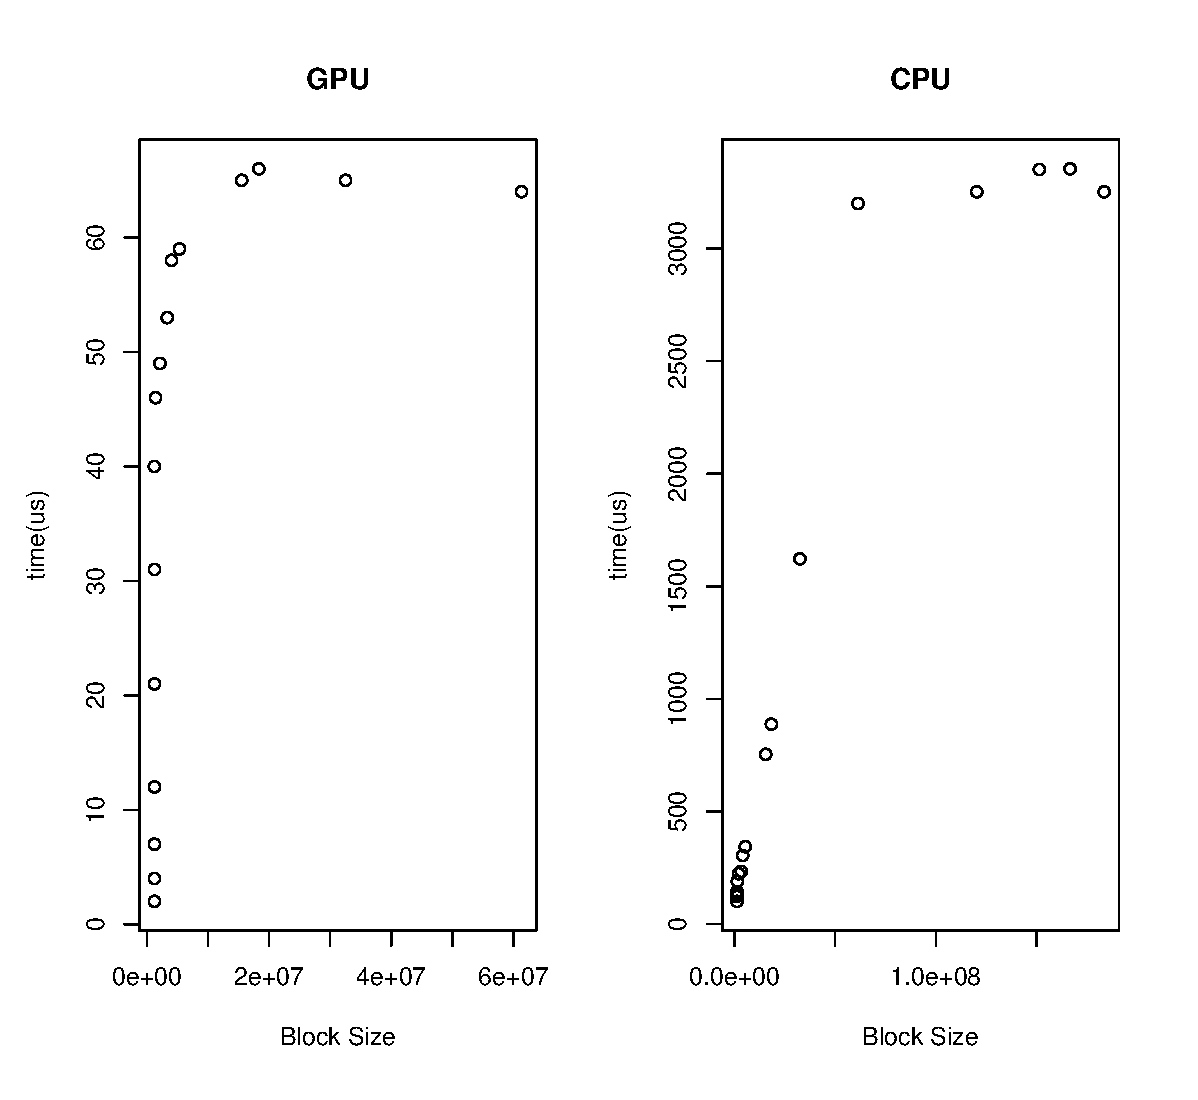
\includegraphics[scale=0.3]{CPUVersusGPU.eps}
	\caption{Curves to GPU x CPU}
	\label{fig:CPUVersusGPU}
	\end{center}
\end{figure*}


Our algorithm determines the optimal block size for each processor using an
iterative process. We initially determine a function $P_p[x]$, which provides
the processing speed for a block of data of size $x$ on processor $p$. The objective of the algorithm is to minimize the total time of the application, by distributing the input data among the processors. The problem can be described as follows:


Suppose we have $n$ processors and a input data size $Z$. We consider that the function of processor $g$ has an input of size $x^g$, corresponding a fraction of input data assigned to processor $g$. In this case, we have $\sum_{g=1}^n x^g = Z$.

We denote as $E^g(x^g)$ the execution time of function in the processor $g$, for input $x^g$. The proposed algorithm consists in fiding the set values:
	
\begin{equation}
	X = \{ x^g \in \mathbb{R}:[0,1] / \sum_{g=1}^n x^g = Z \}
	\label{eq: totalResultado}
\end{equation}

where $g = 1, ..., n$, that minimizes $E^A$ while satisfying  the constraint:

\begin{equation}
	E_{A} = E_{B} = ...= E_{n}
	\label{eq: Restricao}
\end{equation}

which represents that all processors should spend the same amount of time performing  the processing, guaranteeing the execution time of the function in all processors is minimized.

The figure \ref{fig:CPUVersusGPU} shows the curves for a GPU and a CPU, the x-axis we vary the block size and obtained the processing time. It is noticed that the curves are both logarithmic functions. These curves are approximated by the method of \textit{least squares}, which gives us an estimate of the function. The function has the form $f(x) = a ln(x) - b$. The function is constructed performing the execution of small blocks on each processor. 


After generating a certain number of points, normally four points,  a curve is fitted to the points, becoming a model for the processor execution times. We fitted curves for all processors and mount a equation system. We solve a equations system and find a point where minimize the \textit{makespan}. The total execution time spent by each processor $g = \{A, B, C, n\}$, is given by:


\begin{equation}
	T_{g} = E_{A} + E_{B} + E_{C} + ... + E_{n}
	\label{eq: total}
\end{equation}

The \ref{eq: total} is the total execution time, and now we need solve a equation system like this:

\begin{equation}
	\left\{
	\begin{array}{ll}
		\displaystyle x_{1} = a_1 ln(T_1) + b_1\\
		\displaystyle x_{2} = a_2 ln(T_2) + b_2 \\
		\displaystyle x_{n} = a_3 ln(T_n) + b_3 
		\label{eq: system}
	\end{array}
	\right
\end{equation}


The equations system is solve by interior point line search filter method \cite{point}, . From the moment that are generated  the functions by least squares, we continue to measure the time to determine when threads are finishing the job. If the difference of time of threads exceeds a threshold, we restart the process of determining the curves and resolution of the equation system. The synchronization occurs only when the time difference between threads exceeds a threshold set by the user.

Initially the user choose a size block $initialBlockSize$, this size block is send to all processors units. We determine the time for all processors and the processor with smallest time is elected. For the elected processor double the size block and to others units the size block is proportional at time. The proportinal time is calculed getting the time of each processor and divide by faster processor. Next pass is get the size block of faster processor and divide this value by each proportinal time, the resulted is the size block in the next iteration. Each value is plotted and with these values is estimated a funtion through least squares.  A equation system is generated for each processor. The goal is find a size block for all processor that minimize the time and make the processors terminate at the same time. In \ref{alg1} is presented the algorithm. 


\begin{algorithm}

\caption{Dynamic Algorithm}
\label{alg1}

\begin{algorithmic}		

\STATE Function~ dynamic()

\STATE $B \leftarrow initialBlockSize;$
\WHILE{There are data}
	\WHILE{$erroCurve \geq 0.5$}
		\STATE sendPieceDataAllProcessors(B);
		\STATE determineFastesProcessor();
		\STATE dobleFasterProcessor();
	        \STATE calculateProportionalTimeEachProcessor();
		\STATE synchonize();
		\STATE determineCurveProcessor();
	\ENDWHILE
	\STATE solveEquationSystem();
	\STATE $B \leftarrow DistributeBlockSize()$;
	\IF {$timeDiference \geq Threshold$ }
		\STATE synchonize();
		\STATE dynamic();	
    	\ENDIF

\ENDWHILE

\end{algorithmic}
\end{algorithm}

In the algorithm the variable initialBlockSize is initiated by the user. It determines the size of the block in the first iteration for each processor. Then there is a loop that tests whether there are data yet. In the second loop a test is made to determine the error of least squares. We ship the piece of data to all processors, determine the processor that processed the data faster, comparing the processing times. Doubled the time of the faster processor and the other processors sent a piece proportional to the time taken to process the initialBlockSize piece of data, synchronize all processors. And from all values, typically four values ​​of block size and a time equation is determined for each processing unit using the method of least squares. With the equations for each processor the system of equations is solved and distribuited a block size for each processor. If the time difference is increasing with the passage of the distributions is done a synchronization and is rebalanced. The threshold is 0.5 obtained empirically.

%%%%%%%%%%%%%%%%%%%%%%%%%%%%%%%%%%%%%%%%%%%%%%%%%%%%%%%%%%%%%%%%%%%%%%%%%%%

\section{Implementation}

The implementation was done in the C language with the framework StarPU.
StarPU~\cite{starpu} is a tool for parallel programming that supports hybrid
architectures like multicore CPUs and accelerators. The StarPU proposes an
approach of independent tasks based architecture. Codelets are defined as an
abstraction of a task that can be performed on one core of a multicore CPU or
subjected to an accelerator. Each codelet may have multiple implementations, one
for each architecture in which codelet can be performed using specific languages
and libraries for the target architecture. A StarPU application is described as
a set of Codelets with data dependencies.

The tool has a set of scheduling policies implemented that the programmer can
choose according to the characteristics of the application. The main one is the
use of static scheduling algorithm HEFT (Heteregeneous Earliest Finish Time) to
schedule tasks based on cost models of task execution.

For each device one codelet has been programmed with the characteristics of the
devices. A codelet is a structure that represents a computational kernel. Such a
codelet may contain an implementation of the same kernel on different
architectures (e.g. CUDA and x86).  The applications were implemented by
dividing the data set into tasks, implemented as codelets. The tasks are
independent, with each task receiving a part of the input set proportional to
the processor weight. Two Codelets were implemented one for GPU/CUDA and one for
CPU architecture.

To evaluate our load-balancing algorithm, we implemented it by modify the default StarPU balancing algorithm. The modification of the load balancing algorithm is realized by changing the STARPU\_SCHED variable. The STARPU framework has an API that allows modifying the scheduling policies. There are data structures and functions that speed up the process of development. For example the function "double starpu\_timing\_now (void)"  return the current date in micro seconds, which makes it easier for the determination of measures runtime. In StarPU there is a data structure called "starpu\_sched\_policy" This structure contains all the methods que Implement a scheduling policy. 

Three other algorithms were implemented for comparison: the greedy, static and
HDSS. The greedy consisted in dividing the input set in pieces and assigning
each piece of input to any idle processor, without any priority assignment. The
static~\cite{raphael}, measures processing speeds before the execution and set
static block sizes per processor at the beginning of the execution, with the
block size proportional to the processor speed. Finally, The HDSS~\cite{HDSS}
was implemented using minimum square estimation to estimate the weights and
divided into two phases: adaptation phase and completion phase.

The library used for solve the equation system was the IPOPT. IPOPT (Interior Point Optimize) is an open source software package for large-scale nonlinear optimization. It can be used to solve general nonlinear programming problems.

\subsection{Applications}

For evaluating our algorithm, we adapted two applications from the CUDA
SDK~\cite{cuda} to execute using the StarPU framework, the blackscholes and matrix
multiplication applications.

For the matrix multiplication, we assume that each element in the product matrix
can be obtained by applying the equation \ref{eq: matrix}. A copy of the matrix
A was distributed to all processing units and matrix B was divided according to
the load-balancing scheme, the matrix multiplication version use the shared memory. Matrix multiplication has complexity $O(n^3)$.

\begin{equation}
 C[i][j] = \sum_{k=1}^{n}  A[i][k] * B[k][j]
  \label{eq: matrix}
\end {equation}

Blackscholes is a popular financial analysis algorithm for calculating prices
for European style options. The Black-Scholes equation is a differential
equation that describes how, under a certain set of assumptions, the value of an
option changes as the price of the underlying asset changes. More precisely, it
is a stochastic differential equation that includes a random walk term, which
models the random fluctuation of the price of the underlying asset over time.
The Black-Scholes equation implies that the value of a European call option, 
%may be computed as:


%\begin{equation}
 %V = S * C(d_1) - Xe^{-rt} * C(d_2)
  %\label{eq: black}
%\end {equation}

%where:

%\begin{equation}
 %d_1 = \frac {\log {\frac{S}{X}} + T(r + \frac{v^2}{2})}{ v\sqrt{T}}
  %\label{eq: blackD1}
%\end {equation}

%\begin{equation}
 %d_2 =d_1 - v\sqrt{T}
  %\label{eq: blackD2}
%\end {equation}

The cumulative normal distribution function, gives us the probability that a
normally distributed random variable will have a value less than x. There is no
closed-form expression for this function, and as such it must be evaluated
numerically. It is typically approximated using a polynomial function. The idea is to calculate the Black Scholes the greatest amount of possible options. Thus, the input is a vector of data that the options should be calculated by applying the differential equation. The division of the task is given a position of providing input vector to each thread. The complexity of the algorithm is $O(1)$.


%%%%%%%%%%%%%%%%%%%%%%%%%%%%%%%%%%%%%%%%%%%%%%%%%%%%%%%%%%%%%%%%%%%%%%%%%%%

\section{Results}

% RYC: Passei o item "B. System configurations" para o início da seção V, de
% resultados. Normalmente começamos a seção de resultados explicando como os
% experimentos foram realizados. Eu colocaria uma tabela com a descrição das 3
% máquinas, assim fica mais fácil de visualizar.

\subsection{System Configuration}

We used three different machines to evaluate our algorithm. Machine A has a
quad-core: Core i7 CPU, 8 GB of RAM and 2 nVidia GTX 295 board, each GTX 295 has
280 cores per GPU, 999 MHz memory clock and memory bandwidth 223.8 GB/sec with 2
GPUs on each. Machine B has a machine a quad-core Core i7 CPU, 32 GB of RAM and
2 nVidia GTX 680 GPUs, GTX 680 has 1546 cores, 6 Gbps memory clock and memory
bandwidth 192.2 MHz .  Machine C has a machine a quad-core: Core i7 CPU, 32 GB
of RAM and 1 nVidia GTX Titan GPU, GTX Titan has 2688 cores, 6 Gbps memory speed
and memory bandwidth 223.8 GB/sec. We consider the scenarios with only machine
A, with machine A and B, and with the 3 machines (A, B and C). The computers are
connected by a Gigabit Ethernet network. We used Ubuntu 12.04 and CUDA 5.5.

To use all the n multiprocessors from a GPU, it is necessary to create at least
n blocks. Moreover, each multiprocessor simultaneously executes groups (called
warps) of $m$ threads from a single block, and several warps should be present
on each GPU for efficient usage of its processors.

In all tests, we used all the multiprocessor of the GPUs, launching kernels with
$k$ blocks per with 1024 threads for each block, where $k$ is the number of
processor in the GPU. For the used GPUs, $k$ is \textbf{192, 8 and 30} in GTX
Titan, GTX 680 and GTX 295 respectively. For the CPUs, we used all the CPU
cores, launchinhg one task per core.

% RYC: Você precisa colocar também os modelos dos processadores, número de
% núcleos, cache, etc. Enfatize este ponto na seção onde você descreve as
% configurações de hardware e a análise dos resultados.

\subsection{Matrix Multiplication}

We evaluated the execution time of the matrix multiplication application using
one, two and three machines and four different scheduling algorithms: (1) our
algorithm, (2) static, (3) HDSS, and (4) StarPU (greedy). 

\begin{figure*}[htb]
	\begin{center}
	\centering
			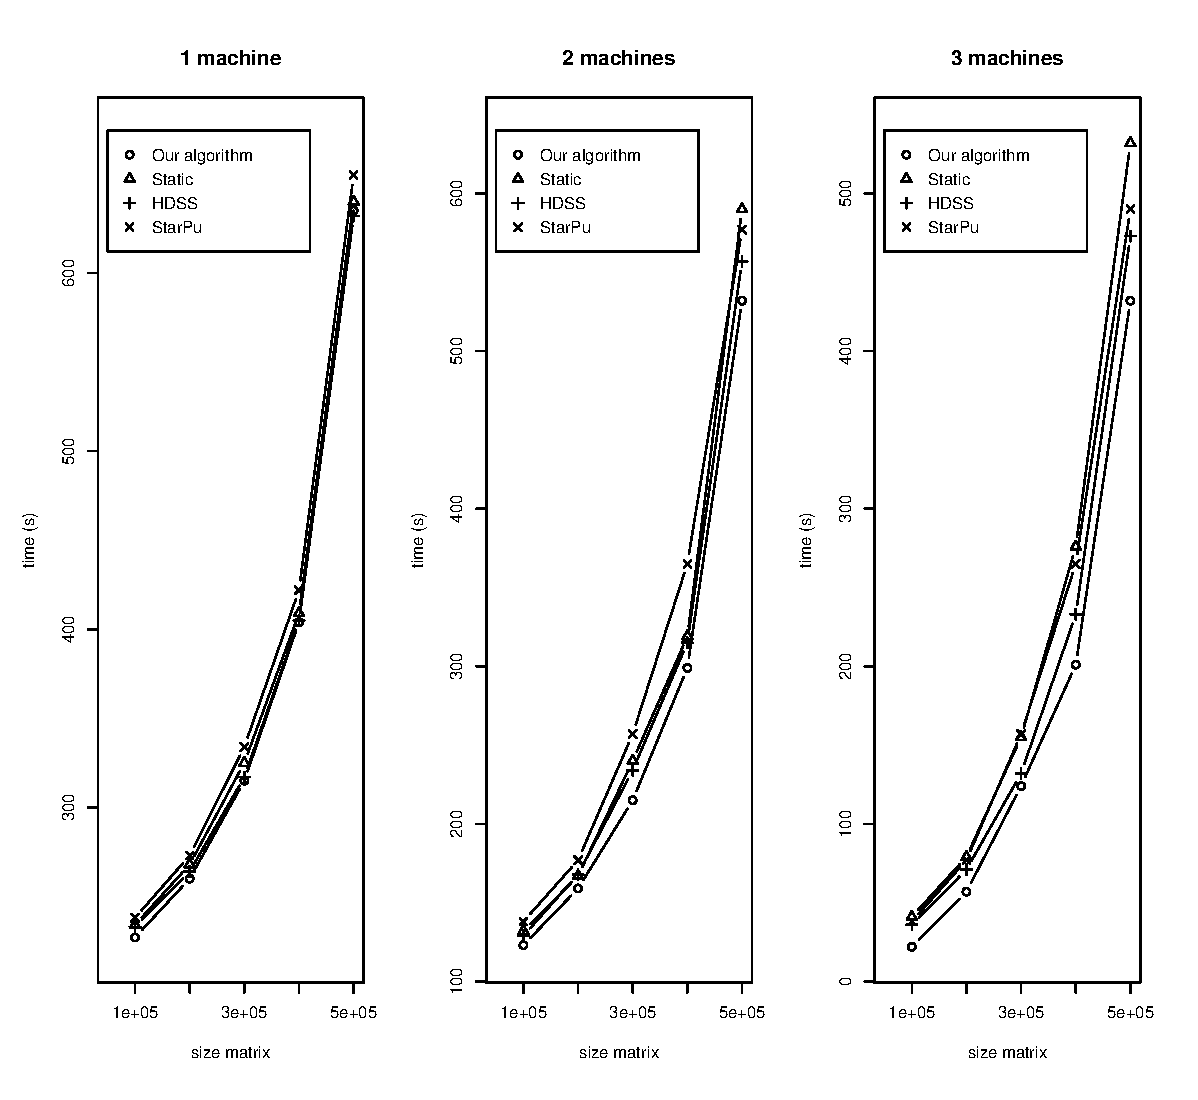
\includegraphics[width=10cm,height=5.8cm]{MaquinasMatrix.eps}
	\caption{Difference in runtime with different sizes of matrices for matrices multiplication}
	\label{fig:todosJuntos}
	\end{center}
\end{figure*}

% RYC: Figuras 1 e 3: Deixar os gráficos mais largos para ocupar a página toda.

% RYC: Quantos execuções você fez para obter cada ponto dos gráficos? Você
% precisa explicitar isto no texto. Coloque também as barras de erro no gráfico.

Figure~\ref{fig:todosJuntos} shows the results for matrices with sizes from
10000 x 10000 to 50000 x 50000. In all scenarios, our scheduling algorithms
obtained the best results, with the HDSS algorithn in second. The static and
StarPU default greedy algorithm were clearly inferior.

With one machine the difference was smaller because there are few types of
devices for the scheduler to select. With two machines our algorithm starts to
perform better, especially for larger matrices, which is explained by the fact
that the execution time of the matrix mutiplication increases quickly as we
increase the matrix size. With three machines we have the most heterogeneous
environment and the performance gain using our algorithm is the largest. As in
the other scenarios, increasing the matrix size also increases the performance
gain with our algorithm.


% RYC: Coloque os números para as matrizes de 10k e 50k explicitamente e a
% diferença em porcentagem. Assim fica mais fácil para o leitor comparar
%
% RYC: O ganho absoluto é maior para matrizes maiores, mas o ganho relativo não
% é similar? Neste caso, nosso algoritmo funciona bem em ambos os casos.


The obtained results shows that the more heterogeneous the environment is, the
largest is the perform advantage of using our proposed algorithm. This advantage
is due to a better distribution of the data along the
execution. Figure~\ref{fig:diferencaThreads} shows the time difference between
the earliest and latest finishing threads, in the scenario with three machines.

\begin{figure*}[htb]
	\begin{center}
	\centering
			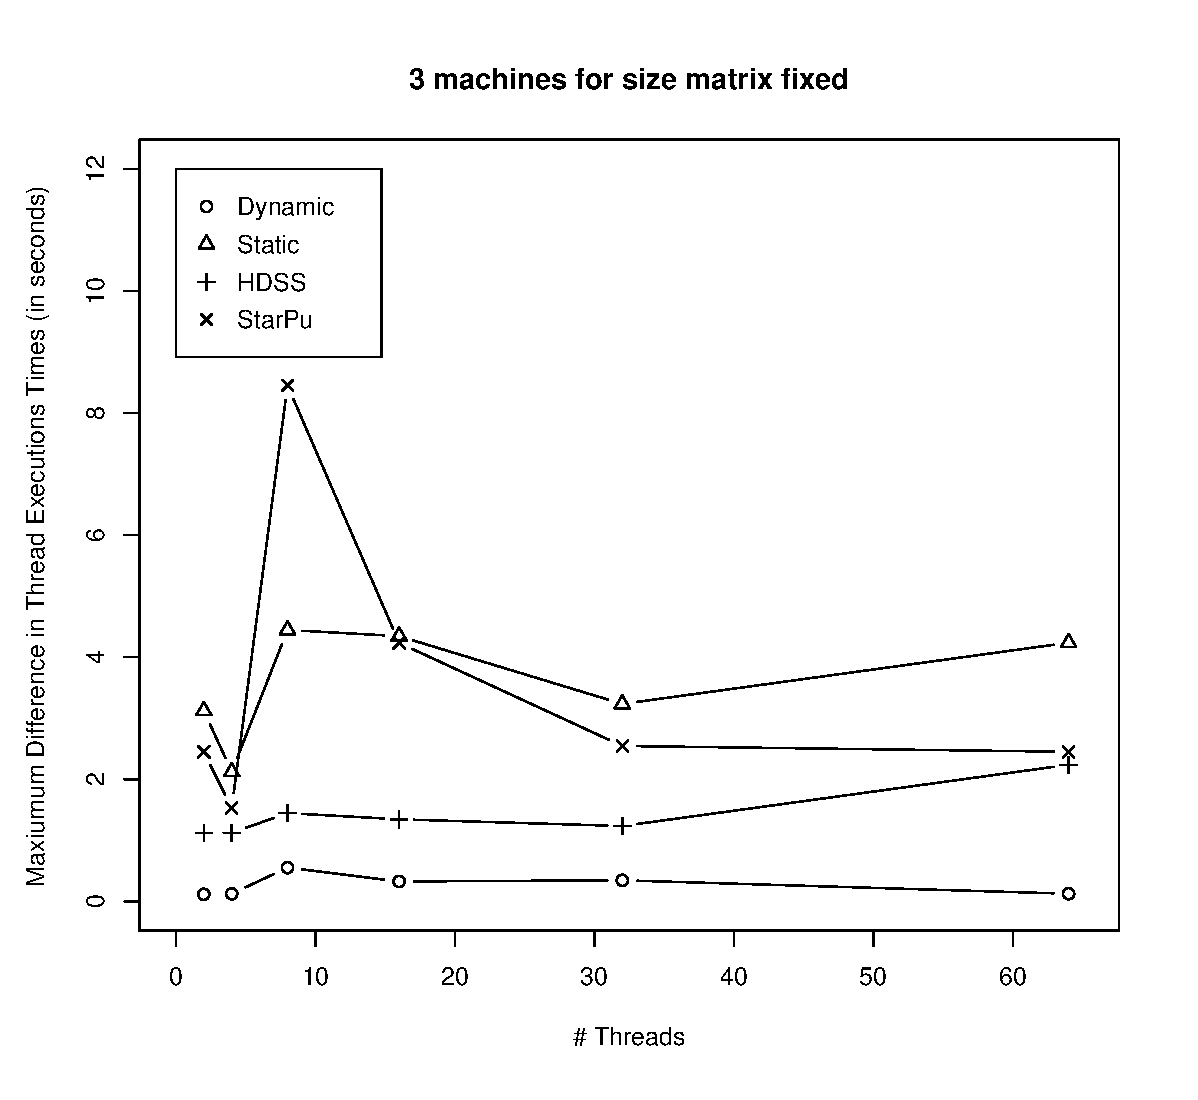
\includegraphics[scale=0.3]{MaximaDiferenca.eps}
	\caption{Time differences between the earliest and latest finishing threads}
	\label{fig:diferencaThreads}
	\end{center}
\end{figure*}

% RYC: Precisa explicar este experimento. Como você fez essa comparação. Para
% cada fase de sincronização você comparou os tempos de todas as threads e pegou
% a diferença e, no final, pegou qual a maior diferença de todas as fases?  

% RYC: As maiores diferenças foram no começo ou no fim da execução? Seria
% interessante um outro gráfico que mostrasse a diferenças médias em toda a
% execução, junto com o desvio padrão. Assim nas figuras 2 e 4 você ficaria com
% 2 gráficos, um com o máximo e outro com as médias.

% RYC: Figuras 2 e 4: you should use the time differences relative to the time
% required to execute the block (for example, time difference / execution
% time). Otherwise, we do not know if a difference of 4 seconds in the execution
% time is large or not.

The StarPU greedy algorithm performed well considering that it do not directly
use information on the processing speeds of the devices. But it uses this
information indirectly, since faster devices finish their tasks earlier and,
consequently, receive more tasks. The static algorithm (...)

% RYC: Por que o desempenho do algoritmo estático foi tão ruim? Ele não é
% similar ao dinâmico?

HDSS uses the beginning of the execution to estimate the best block size
distribution and uses this distribution through the complete
execution. Moreover, larger blocks are used in the beginning of the execution,
causing a larger delay due to disbalance when use different types of devices,
such as GPUs and CPUs. Finally, HDSS uses a crude approxiamtion to the device
capabilities.

Our algorithm estimate fairly accurately the amount of data that should be
provided to each processing unit, solving an optimization problem with the
restriction that all units should finish the execution of the tasks at the same
time. When the difference between finishing the execution of threads for certain
data partition exceeds a certain threshold, the algorithm rebalances the data
distribution.

%---------------------------------------------------------------------------
\subsection{Blackscholes}

\begin{figure*}[htb]
	\begin{center}
	\centering
			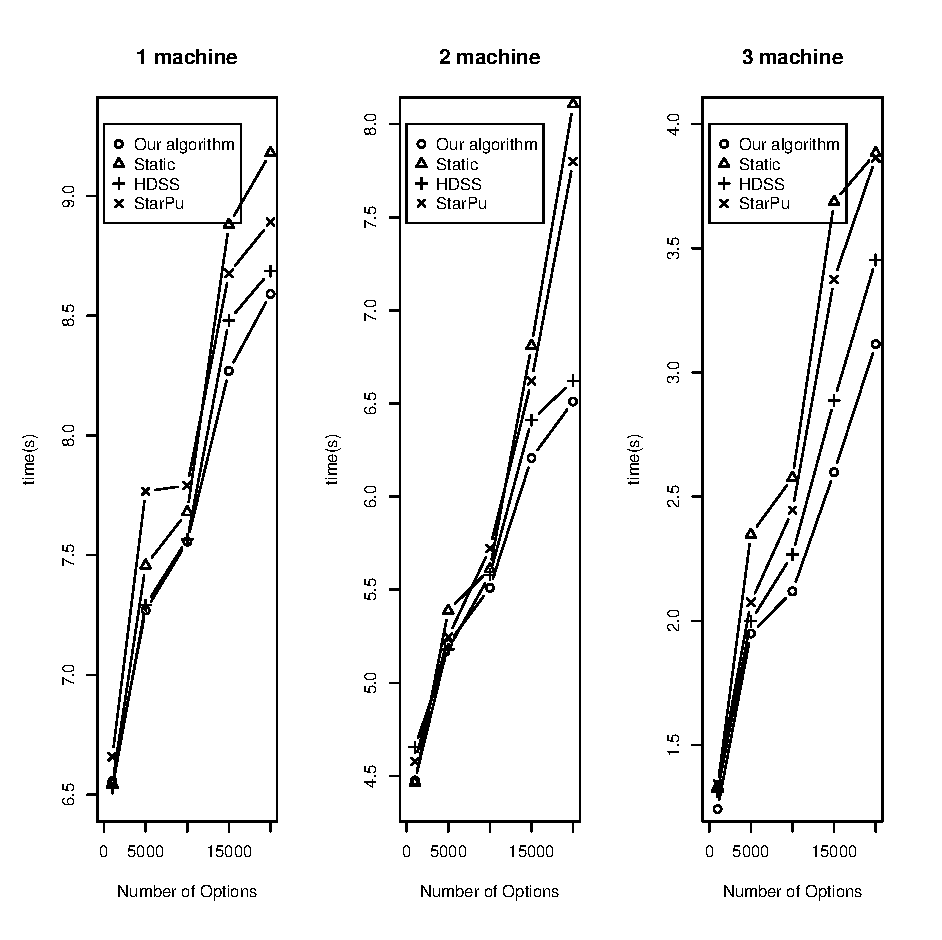
\includegraphics[width=10cm,height=5.8cm]{MaquinaBlack.eps}
	\caption{Difference in runtime with different number options}
	\label{fig:black}
	\end{center}
\end{figure*}

We evaluate the execution time of the Blackscholes application using different
machine configurations. Figure~\ref{fig:black} shows the execution times, where
we varied the number of options on each execution and obtained the
runtimes. Similarly to the matrix multiplication experiments, the performance
gains were the largest with bigger problem sizes (number of options) and more
heterogeneous environments, and the results can be explained using the same
arguments. Interestingly, the Blackscholes application has linear complexity
with the number of options, showing that our scheduling algorithm is also useful
with this class of application.

% RYC: Colocar alguns valores explicitamente, com a diferença de desempenho em
% porcentagem. Assim fica mais fácil para o leitor comparar os resultados

Also, considering that the application finishes in less than 4 seconds, for the
scenario with 3 machines, we also see that the cost of solving the optimization
problem to determine the best data distribution is small and the obtained gains
outweighs the cost of the calculations. For applications tested in a few
iterations around 6, it was possible to obtain the solution of the system in a
few milisseconds.

% RYC: Você tem uma estimativa do tempo necessário para calcular a distribuição?
% É realmente da ordem de milisegundos?

\begin{figure*}[htb]
	\begin{center}
	\centering
			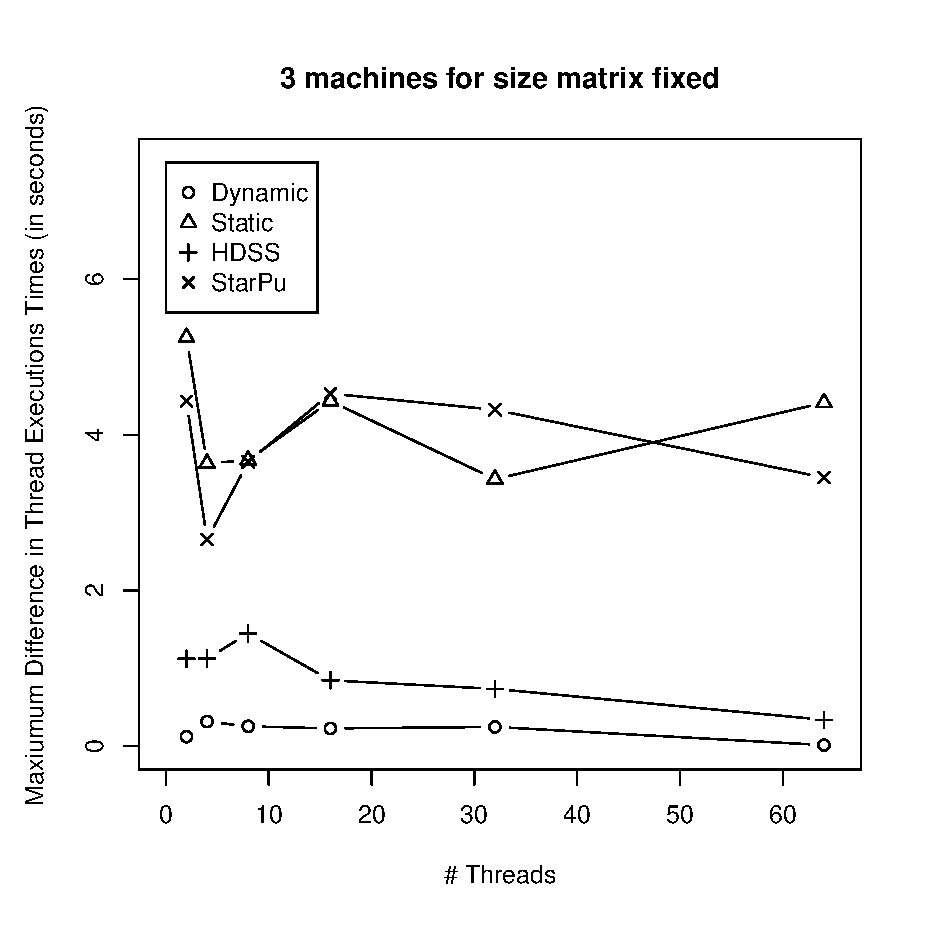
\includegraphics[scale=0.4]{MaximaDiferencaBlack.eps}
	\caption{Time differences between the earliest and latest finishing threads}
	\label{fig:diferencaThreadsBlack}
	\end{center}
\end{figure*}

Figure~\ref{fig:diferencaThreadsBlack} confirms this result, showing that the
time difference between the earliest and latest finishing threads, in the
scenario with three machines is always smaller for our proposed algorithm.

%-------------------------------------------------------------------------------
\section{Conclusions and future work}

In this paper we propose an algorithm for scheduling tasks in domain
decomposition problems executing on clusters of heterogeneous CPUs and GPUs. It
outperforms other similar existing algorithms, due to the online estimation of
the performance curve for each processing unit and the selection of the best
data distribution for the devices. We showed for two applications that our
algorithm provides the highest gains for more heterogeneous and larger problems
sizes.

Although we used dedicated clusters, we can also consider the usage of public
clouds, where the user can request a number of resources allocated in virtual
machines from shared machines. In this case, the quality of service may change
during execution, and the addition of the execution time difference threshold
permits readjustments in data distributions. We can also consider the scenario
with added fault-tolerance, where machines may become unavailable during
execution. In this scenario, a simple redistribution of the data among the
remaining devices would permit the application to readapt to this scenario.

As ongoing work, we are including the cost of communication in the scheduling
algorithm, which is essential for applications where the time spent with
information exchange among the tasks cannot be ignored.

% use section* for acknowledgement
\section*{Acknowledgment}


The authors would like to thank FAPESP (Proc. n. 2012/03778-0) for the financial support.


\ifCLASSOPTIONcaptionsoff
  \newpage
\fi

% can use a bibliography generated by BibTeX as a .bbl file
% BibTeX documentation can be easily obtained at:
% http://www.ctan.org/tex-archive/biblio/bibtex/contrib/doc/
% The IEEEtran BibTeX style support page is at:
% http://www.michaelshell.org/tex/ieeetran/bibtex/
\bibliographystyle{IEEEtran}
% argument is your BibTeX string definitions and bibliography database(s)
%\bibliography{IEEEabrv,../bib/paper}
%
% <OR> manually copy in the resultant .bbl file
% set second argument of \begin to the number of references
% (used to reserve space for the reference number labels box)
% File .bib
\bibliography{article}


\end{document}


